\documentclass[10pt,conference]{IEEEtran}
% SANER 2027 Short Papers and Posters: IEEEtran conference, no compsoc; 6 pages INCLUDING references.
\usepackage{cite}
\usepackage{amsmath}
\usepackage{array}
\usepackage{url}
\usepackage{tikz}
\usetikzlibrary{arrows.meta,calc,positioning}
\usepackage[hidelinks]{hyperref}
\hypersetup{pdfauthor={},pdftitle={Cohort versus Per-Item Coding-Agent Execution of Coupled Work Items: Early Results},pdfsubject={},pdfkeywords={},pdfcreator={},pdfproducer={}}

% Every result number in the prose comes from these generated files.
% Generated by scripts/build_tables.py from data/metrics.json. Do not edit.
% Numbers only (no units or % signs). Lower bounds carry \ensuremath{\geq}.
% Reductions are percentages; ratios are independent/grouped.
\newcommand{\AcostGrouped}{9.48} % A021 platform cost USD, grouped
\newcommand{\AcostIndep}{21.51} % A021 platform cost USD, independent
\newcommand{\AcostRatio}{2.27} % A021 platform cost, independent/grouped
\newcommand{\AcostReduction}{56.0} % A021 platform cost, grouped reduction in percent
\newcommand{\AoutputGrouped}{112,377} % A021 platform output tokens, grouped
\newcommand{\AoutputIndep}{244,630} % A021 platform output tokens, independent
\newcommand{\AoutputRatio}{2.18} % A021 platform output tokens, independent/grouped
\newcommand{\AoutputReduction}{54.1} % A021 platform output tokens, grouped reduction in percent
\newcommand{\AcacheReadGrouped}{24.51} % A021 platform cache-read tokens, millions, grouped
\newcommand{\AcacheReadIndep}{45.07} % A021 platform cache-read tokens, millions, independent
\newcommand{\AcacheReadRatio}{1.84} % A021 platform cache-read tokens, independent/grouped
\newcommand{\AcacheReadReduction}{45.6} % A021 platform cache-read tokens, grouped reduction in percent
\newcommand{\AactiveMinGrouped}{61.2} % A021 active session time, minutes, grouped
\newcommand{\AactiveMinIndep}{111.4} % A021 active session time, minutes, independent
\newcommand{\AactiveRatio}{1.82} % A021 active session time, independent/grouped
\newcommand{\AactiveReduction}{45.1} % A021 active session time, grouped reduction in percent
\newcommand{\AspanMinGrouped}{61.2} % A021 wall-clock span, minutes, grouped
\newcommand{\AspanMinIndep}{292.1} % A021 wall-clock span, minutes, independent
\newcommand{\AspanHmIndep}{4:52} % A021 wall-clock span, independent, h:mm
\newcommand{\AspanRatio}{4.77} % A021 wall-clock span, independent/grouped
\newcommand{\AspanReduction}{79.1} % A021 wall-clock span, grouped reduction in percent
\newcommand{\AblockedMinIndep}{127.1} % A021 permission-block time, minutes
\newcommand{\AsessionsGrouped}{1} % A021 implementation sessions, grouped
\newcommand{\AsessionsIndep}{5} % A021 implementation sessions, independent
\newcommand{\AfailedAttemptsIndep}{2} % A021 failed attempt sessions
\newcommand{\AmodelRequestsGrouped}{\ensuremath{\geq}114} % A021 model requests (script; independent is a lower bound), grouped
\newcommand{\AmodelRequestsIndep}{\ensuremath{\geq}237} % A021 model requests (script; independent is a lower bound), independent
\newcommand{\AfileReadsGrouped}{\ensuremath{\geq}52} % A021 file reads (script; independent lower bound), grouped
\newcommand{\AfileReadsIndep}{\ensuremath{\geq}134} % A021 file reads (script; independent lower bound), independent
\newcommand{\AsearchesGrouped}{\ensuremath{\geq}53} % A021 searches (script; independent lower bound), grouped
\newcommand{\AsearchesIndep}{\ensuremath{\geq}159} % A021 searches (script; independent lower bound), independent
\newcommand{\AbuildsGrouped}{\ensuremath{\geq}16} % A021 build commands (script), grouped
\newcommand{\AbuildsIndep}{\ensuremath{\geq}34} % A021 build commands (script), independent
\newcommand{\AtestRunsGrouped}{\ensuremath{\geq}13} % A021 test-run commands (script), grouped
\newcommand{\AtestRunsIndep}{\ensuremath{\geq}15} % A021 test-run commands (script), independent
\newcommand{\AagentsReadsGrouped}{\ensuremath{\geq}1} % A021 AGENTS.md reads, grouped
\newcommand{\AagentsReadsIndep}{\ensuremath{\geq}5} % A021 AGENTS.md reads, independent
\newcommand{\AgovReadsGrouped}{\ensuremath{\geq}6} % A021 governance/planning reads, grouped
\newcommand{\AgovReadsIndep}{\ensuremath{\geq}15} % A021 governance/planning reads, independent
\newcommand{\AfirstCodeMinGrouped}{9.6} % A021 summed time to first code change, minutes, grouped
\newcommand{\AfirstCodeMinIndep}{\ensuremath{\geq}21.5} % A021 summed time to first code change, minutes, independent
\newcommand{\AcontextKGrouped}{318.8} % A021 largest end-of-session context, k tokens, grouped
\newcommand{\AcontextKIndep}{262.8} % A021 largest end-of-session context, k tokens, independent
\newcommand{\AtestsGrouped}{811} % A021 final F\# tests passed, grouped
\newcommand{\AtestsIndep}{829} % A021 final F\# tests passed, independent
\newcommand{\AtestsAddedGrouped}{19} % A021 work-group tests added (evaluation 1), grouped
\newcommand{\AtestsAddedIndep}{37} % A021 work-group tests added (evaluation 1), independent
\newcommand{\AkitDefectsGrouped}{0} % A021 kit-evaluation defect findings, grouped
\newcommand{\AkitDefectsIndep}{2} % A021 kit-evaluation defect findings, independent
\newcommand{\AmergeConflictsGrouped}{0} % A021 merges with conflicts, grouped
\newcommand{\AmergeConflictsIndep}{1} % A021 merges with conflicts, independent
\newcommand{\RtwoCostGrouped}{10.75} % R2 platform cost USD, workers, grouped
\newcommand{\RtwoCostIndep}{22.56} % R2 platform cost USD, workers, independent
\newcommand{\RtwoCostRatio}{2.10} % R2 platform cost, workers, independent/grouped
\newcommand{\RtwoCostReduction}{52.3} % R2 platform cost, workers, grouped reduction in percent
\newcommand{\RtwoOutputGrouped}{132,902} % R2 platform output tokens, workers, grouped
\newcommand{\RtwoOutputIndep}{236,654} % R2 platform output tokens, workers, independent
\newcommand{\RtwoOutputRatio}{1.78} % R2 platform output tokens, workers, independent/grouped
\newcommand{\RtwoOutputReduction}{43.8} % R2 platform output tokens, workers, grouped reduction in percent
\newcommand{\RtwoCacheReadGrouped}{27.91} % R2 platform cache-read tokens, millions, workers, grouped
\newcommand{\RtwoCacheReadIndep}{54.49} % R2 platform cache-read tokens, millions, workers, independent
\newcommand{\RtwoCacheReadRatio}{1.95} % R2 platform cache-read tokens, workers, independent/grouped
\newcommand{\RtwoCacheReadReduction}{48.8} % R2 platform cache-read tokens, workers, grouped reduction in percent
\newcommand{\RtwoActiveMinGrouped}{55.9} % R2 active session time, workers, minutes, grouped
\newcommand{\RtwoActiveMinIndep}{100.5} % R2 active session time, workers, minutes, independent
\newcommand{\RtwoActiveRatio}{1.80} % R2 active session time, workers, independent/grouped
\newcommand{\RtwoActiveReduction}{44.4} % R2 active session time, workers, grouped reduction in percent
\newcommand{\RtwoSpanMinGrouped}{55.9} % R2 wall-clock span, workers, minutes, grouped
\newcommand{\RtwoSpanMinIndep}{133.3} % R2 wall-clock span, workers, minutes, independent
\newcommand{\RtwoSpanRatio}{2.38} % R2 wall-clock span, workers, independent/grouped
\newcommand{\RtwoSpanReduction}{58.1} % R2 wall-clock span, workers, grouped reduction in percent
\newcommand{\RtwoCostInclOrchIndep}{26.05} % R2 platform cost USD, independent incl. orchestrator
\newcommand{\RtwoOrchCostIndep}{3.49} % R2 independent-arm orchestrator cost USD
\newcommand{\RtwoCostInclOrchRatio}{2.4224} % R2 platform cost incl. orchestrator, independent/grouped
\newcommand{\RtwoCostInclOrchReduction}{58.72} % R2 platform cost incl. orchestrator, grouped reduction in percent
\newcommand{\RtwoOutputInclOrchRatio}{1.9781} % R2 output tokens incl. orchestrator, independent/grouped
\newcommand{\RtwoOutputInclOrchReduction}{49.45} % R2 output tokens incl. orchestrator, grouped reduction in percent
\newcommand{\RtwoCacheReadInclOrchRatio}{2.2557} % R2 cache-read incl. orchestrator, independent/grouped
\newcommand{\RtwoCacheReadInclOrchReduction}{55.67} % R2 cache-read incl. orchestrator, grouped reduction in percent
\newcommand{\RtwoElapsedGrouped}{0h55m53s} % R2 elapsed as reported, grouped
\newcommand{\RtwoElapsedIndep}{2h23m35s} % R2 elapsed as reported, independent
\newcommand{\RtwoElapsedRatio}{2.5693} % R2 elapsed as reported (wall-clock incl. orchestration), independent/grouped
\newcommand{\RtwoElapsedReduction}{61.08} % R2 elapsed as reported (wall-clock incl. orchestration), grouped reduction in percent
\newcommand{\RtwoSessionsGrouped}{1} % R2 implementation sessions, grouped
\newcommand{\RtwoSessionsIndep}{5} % R2 implementation sessions, independent
\newcommand{\RtwoModelRequestsGrouped}{\ensuremath{\geq}126} % R2 model requests (script), grouped
\newcommand{\RtwoModelRequestsIndep}{\ensuremath{\geq}343} % R2 model requests (script), independent
\newcommand{\RtwoFileReadsGrouped}{\ensuremath{\geq}69} % R2 file reads (script), grouped
\newcommand{\RtwoFileReadsIndep}{\ensuremath{\geq}185} % R2 file reads (script), independent
\newcommand{\RtwoSearchesGrouped}{\ensuremath{\geq}98} % R2 searches (script), grouped
\newcommand{\RtwoSearchesIndep}{\ensuremath{\geq}208} % R2 searches (script), independent
\newcommand{\RtwoAgentsReadsGrouped}{\ensuremath{\geq}2} % R2 AGENTS.md reads, grouped
\newcommand{\RtwoAgentsReadsIndep}{\ensuremath{\geq}8} % R2 AGENTS.md reads, independent
\newcommand{\RtwoGovReadsGrouped}{\ensuremath{\geq}8} % R2 governance/planning reads, grouped
\newcommand{\RtwoGovReadsIndep}{\ensuremath{\geq}34} % R2 governance/planning reads, independent
\newcommand{\RtwoFirstCodeMinGrouped}{9.4} % R2 summed time to first code change, minutes, grouped
\newcommand{\RtwoFirstCodeMinIndep}{34.2} % R2 summed time to first code change, minutes, independent
\newcommand{\RtwoTestsGrouped}{819} % R2 final F\# tests passed, grouped
\newcommand{\RtwoTestsIndep}{839} % R2 final F\# tests passed, independent
\newcommand{\RtwoTestsAddedGrouped}{27} % R2 net F\# tests added vs baseline, grouped
\newcommand{\RtwoTestsAddedIndep}{47} % R2 net F\# tests added vs baseline, independent
\newcommand{\RtwoDefectsGrouped}{2} % R2 confirmed acceptance defects, grouped
\newcommand{\RtwoDefectsIndep}{2} % R2 confirmed acceptance defects, independent
\newcommand{\RtwoMergeConflictsGrouped}{0} % R2 merges with conflicts, grouped
\newcommand{\RtwoMergeConflictsIndep}{2} % R2 merges with conflicts, independent
\newcommand{\BaselineTests}{792} % F\# tests at the shared baseline
\newcommand{\AcostReductionExclFailed}{46.4} % A021 platform cost, grouped reduction in percent, excluding failed attempts
\newcommand{\AactiveReductionExclFailed}{30.7} % A021 active session time, grouped reduction in percent, excluding failed attempts

% Generated by scripts/build_architecture_table.py from data/architecture-findings.json and data/metrics.json. Do not edit.
\newcommand{\ArchDimensions}{eight} % rubric dimensions
\newcommand{\ArchFindings}{32} % coded findings (study x arm x dimension)
\newcommand{\ArchCitations}{100} % code citations verified
\newcommand{\ArchFalsificationAttempts}{12} % falsification attempts


\newcommand{\G}{G}
\newcommand{\I}{I}

\begin{document}

\title{Cohort versus Per-Item Coding-Agent Execution of Coupled Work Items: Early Results from a Case Study and an Internal Re-Execution}

\author{\IEEEauthorblockN{Anonymous Author(s)}\IEEEauthorblockA{Anonymous Institution(s)}}

\maketitle

\begin{abstract}
Coding agents usually get one work item per fresh session, even when items share design decisions. We executed five coupled work items of an F\#/.NET command-line tool in two ways: \G, one session that first writes and commits a mandated cross-item analysis and then implements all items; and \I, five fresh sessions run serially on one branch, whose prompts neither frame the items as a cohort nor request cross-item analysis. % CLAIM: C01
The arms differ in retained context and in the instructed analysis, and every session's repository contained the study's hypothesis and cohort labels. % CLAIM: C02 C52
In an original study and an internal, non-preregistered re-execution (one execution per arm each), \I{} used about \AcostRatio$\times$ and \RtwoCostRatio$\times$ the worker-only platform cost of \G, a gap that includes per-session overhead and that single runs cannot separate from run-to-run variation. % CLAIM: C11 C13 C60 C61
On a post hoc rubric coded by one AI auditor, \G{} applied one rule where \I{} diverged on member admission, the error and exit-code contract and write locking in both studies, although \I's admission difference follows the acceptance criteria; \I{} validated checkpoint ownership better. Both arms had defects. We report these as hypotheses for a preregistered three-arm study. % CLAIM: C21 C22 C53 C23 C34
\end{abstract}

% ======================================================================
\section{Introduction}

Issue-resolution benchmarks and common practice give an agent one work item per fresh session~\cite{jimenez2024swebench}. When items share a domain model, persistence and command conventions, separate sessions may settle those shared invariants differently; one long session may settle them once but lose per-item detail~\cite{liu2024lost}. That partitioning coupled work across agents changes outcomes is known~\cite{khatua2026cooperbench,ren2026coordination}, as is that grouping tasks in one call cuts cost~\cite{cheng2023batch}. We report early observations on a narrower, common partition: \emph{serial, non-communicating fresh sessions on one branch} versus \emph{one cohort session with a mandated analysis}, on real repository work, measuring cross-item consistency next to cost and per-item correctness, in two executions.

\textbf{Related work.} CooperBench found that one agent implementing two coupled features outperformed two communicating agents~\cite{khatua2026cooperbench}; MSEval varies collaboration topology~\cite{ren2026coordination}; CAID finds that isolated workspaces with structured merging can beat a single agent~\cite{geng2026caid}. Carried-over state can also propagate errors~\cite{shen2026evocode}. Our split sessions differ from these: they run serially, do not communicate and share only the branch. Plan-then-execute prompting~\cite{wang2023plan} resembles our cohort arm's mandated analysis, which is one reason our treatment is a bundle. Reporting guidance for LLM-based SE studies asks for human validation~\cite{wagner2025towards}, which our rubric lacks.

% ======================================================================
\section{Study Design}

\textbf{Subject and cohort.} The subject is an F\#/.NET command-line tool that governs repository work items and includes a planner that rates item affinity from explicit shared signals (paths, tags, dependencies). Five items add a \texttt{work group} command family: create (1), show (2), add (3), remove (4), checkpoint (5). The planner rated them high affinity and mutually conflicting, so \I's sessions ran serially. % CLAIM: C05
Their acceptance criteria require the execution-repository check at add but not at create. % CLAIM: C53
The items were written by AI agents of the product that designed and ran the study. % CLAIM: C41

\textbf{Treatments.} All arms branch from one baseline commit (Fig.~\ref{fig:design}). All implementation sessions ran a Claude Opus-family model in the Claude Code remote runtime. % CLAIM: C03 C10
\G's prompt requires reading every item and the planner's group explanation and, before any code change, committing an analysis of common architecture, shared invariants and reusable abstractions. \I's five prompts each name one item and request no cross-item analysis. % CLAIM: C01
Because \G{} was asked for shared invariants and is then scored on them, the consistency outcome partly measures compliance with an instruction only \G{} received. % CLAIM: C59
\textbf{Contamination.} The baseline every session checked out contained the hypothesis, the protocol and planner outputs; every item text named the experiment cohort and its dependencies; \I's prompts named \G's branch as one not to read. Transcripts were not retained, so exposure is unknown: a major demand-characteristics threat for both arms. % CLAIM: C52

\begin{figure}[t]
\centering
% Study design flow (Fig. 1). TikZ; no data values. Explicit coordinates (column width).
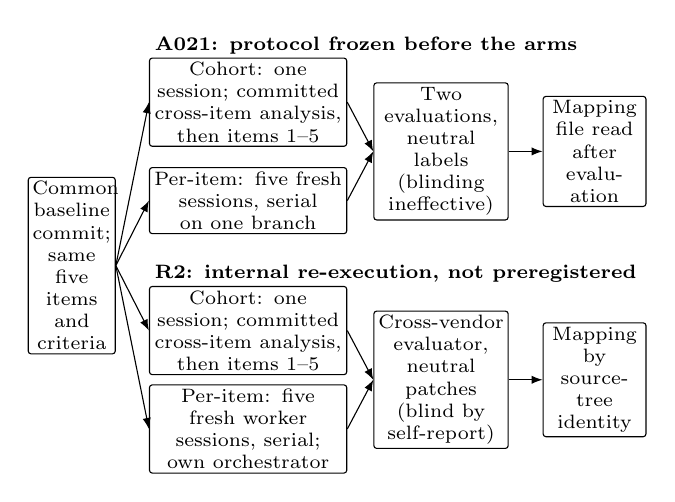
\begin{tikzpicture}[
  font=\scriptsize,
  box/.style={draw, rounded corners=1pt, align=center, inner sep=1.5pt, minimum height=6mm},
  arm/.style={box, anchor=west, text width=24mm},
  eval/.style={box, anchor=west, text width=16mm},
  rev/.style={box, anchor=west, text width=12mm},
  study/.style={font=\scriptsize\bfseries, anchor=west},
  arr/.style={-{Latex[length=1.4mm]}, thin}]
  % rows: A021 cohort, A021 per-item, R2 cohort, R2 per-item
  \node[study] at (1.55, 0.72) {A021: protocol frozen before the arms};
  \node[arm] (ag) at (1.6, 0.0) {Cohort: one session; committed cross-item analysis, then items 1--5};
  \node[arm] (ai) at (1.6, -1.25) {Per-item: five fresh sessions, serial on one branch};
  \node[eval] (ae) at (4.45, -0.625) {Two evaluations, neutral labels (blinding ineffective)};
  \node[rev] (ar) at (6.6, -0.625) {Mapping file read after evaluation};
  \node[study] at (1.55, -2.18) {R2: internal re-execution, not preregistered};
  \node[arm] (rg) at (1.6, -2.9) {Cohort: one session; committed cross-item analysis, then items 1--5};
  \node[arm] (ri) at (1.6, -4.15) {Per-item: five fresh worker sessions, serial; own orchestrator};
  \node[eval] (re) at (4.45, -3.525) {Cross-vendor evaluator, neutral patches (blind by self-report)};
  \node[rev] (rr) at (6.6, -3.525) {Mapping by source-tree identity};
  % common baseline
  \node[box, text width=10mm] (b) at (0.62, -2.075) {Common baseline commit; same five items and criteria};
  \foreach \t in {ag, ai, rg, ri} \draw[arr] (b.east) -- (\t.west);
  \foreach \s/\e in {ag/ae, ai/ae, rg/re, ri/re} \draw[arr] (\s.east) -- (\e.west);
  \draw[arr] (ae) -- (ar);
  \draw[arr] (re) -- (rr);
\end{tikzpicture}

\caption{Design of both studies: one execution per arm per study from one baseline.}
\label{fig:design}
\end{figure}

\textbf{Studies.} The original study (A021) followed a protocol frozen before the arms. % CLAIM: C04
Its \I{} arm needed seven sessions: item 4's first attempt stalled with nothing pushed; the second implemented the item and then blocked on a permission prompt; a third did bookkeeping. % CLAIM: C37
The re-execution (R2) reused baseline, cohort, criteria and model, but changed the evaluator, prompts (not archived), orchestration and metric definitions; it was not preregistered and its designer knew A021's interim results. % CLAIM: C08 C09
\textbf{Evaluation.} The A021 evaluations used neutral labels but were not effectively blind (arm names in commit history; an evaluator reported knowing the mapping). R2's evaluator, an OpenAI GPT-family model, was blind by self-report only. % CLAIM: C06 C07
\textbf{Measures.} Worker-only platform cost and summed session time (all sessions that worked on an arm's items, without orchestrators or evaluators); transcript counts, which are lower bounds in both arms; and an eight-dimension rubric written after unblinding, coded by one AI auditor with code citations and runtime probes, with no second coder. % CLAIM: C11 C18 C58 C29
We report no statistics: one execution per arm, dependent items.

% ======================================================================
\section{Results}

% Generated by scripts/build_tables.py from data/metrics.json. Do not edit.
\begin{table}[t]
\centering
\scriptsize
\setlength{\tabcolsep}{2.5pt}
\caption{Worker-only resources and lower-bound repeated-context counts, one execution per arm}
\label{tab:resources-compact}
\begin{tabular}{@{}p{0.33\columnwidth}rrrrrr@{}}
\hline
 & \multicolumn{3}{c}{A021} & \multicolumn{3}{c}{R2} \\
Measure & G & I & I/G & G & I & I/G \\
\hline
Cost, platform (USD) & 9.48 & 21.51 & 2.3 & 10.75 & 22.56 & 2.1 \\
Output tokens, platform (k) & 112.4 & 244.6 & 2.2 & 132.9 & 236.7 & 1.8 \\
Cache-read tokens, platform (M) & 24.51 & 45.07 & 1.8 & 27.91 & 54.49 & 2.0 \\
Active session time, sum (min) & 61.2 & 111.4 & 1.8 & 55.9 & 100.5 & 1.8 \\
Lines inserted, src+tests+docs & 2,279 & 4,048 & -- & 2,309 & 3,223 & -- \\
of which in tests & 517 & 930 & -- & 686 & 1,113 & -- \\
Model requests, script & $\geq$114 & $\geq$237 & -- & $\geq$126 & $\geq$343 & -- \\
File reads, script & $\geq$52 & $\geq$134 & -- & $\geq$69 & $\geq$185 & -- \\
Searches, script & $\geq$53 & $\geq$159 & -- & $\geq$98 & $\geq$208 & -- \\
\hline
\end{tabular}

\vspace{2pt}\parbox{\columnwidth}{\scriptsize Workers: every session that worked on an arm's items, including the extra item-4 sessions in A021; orchestrators and evaluators excluded. $\geq$: lower bound (script run before each session's final steps; no ratio computed). Single executions: ratios are observations, not effect estimates.}
\end{table}


\textbf{Resources.} \I{} used about \AcostRatio$\times$ (A021) and \RtwoCostRatio$\times$ (R2) the worker-only cost of \G{} and about \AactiveRatio$\times$ and \RtwoActiveRatio$\times$ the summed session time (Table~\ref{tab:resources-compact}). % CLAIM: C11 C13 C12 C14
Without A021's stalled attempt the cost ratio is about \AcostExclStalledRatio$\times$. % CLAIM: C17
Part of the gap is per-session overhead (each fresh session installed the toolchain and read the instructions), and agent token use varies widely across identical runs~\cite{bai2026tokens}, so these are observations, not effect estimates. % CLAIM: C60 C61
The lower-bound counts of requests, reads and searches were smaller for \G{} in both studies; no session compacted. % CLAIM: C18 C20

% Generated by scripts/build_architecture_table.py from data/architecture-findings.json and data/metrics.json. Do not edit.
\begin{table}[t]
\centering
\scriptsize
\setlength{\tabcolsep}{3pt}
\caption{Architecture rubric: category per arm and direction per study}
\label{tab:architecture}
\begin{tabular}{@{}p{0.40\columnwidth}cccc@{}}
\hline
 & \multicolumn{2}{c}{A021} & \multicolumn{2}{c}{R2} \\
Dimension & G/I & Dir. & G/I & Dir. \\
\hline
D1 Persistence/store model & U/DC & G & U/DC & G \\
D2 Member admission (create vs.\ add) & U/Dv & G$^{b}$ & U/Dv & G$^{b}$ \\
D3 Member classification (show vs.\ checkpoint) & U/Dv$^{\dagger}$ & G$^{b}$ & Dv/Dv$^{\dagger}$ & eq \\
D4 Checkpoint ownership validation & Mi/U$^{\dagger}$ & I$^{b}$ & Mi/U & I$^{b}$ \\
D5 Error/JSON/exit contract & U/Dv & G$^{b}$ & U/Dv & G$^{b}$ \\
D6 Mutation/concurrency model & U/Dv & G$^{b}$ & U/Dv & G$^{b}$ \\
D7 Reuse of baseline rules & Dv/U & mixed$^{b}$ & Dv/U & mixed$^{b}$ \\
D8 Incompatible duplicates in feature & U/DC$^{\dagger}$ & G & U/U & eq \\
\hline
\multicolumn{5}{@{}l}{A021 tally: G more unified 6 (4 behavioral), I more unified 1, mixed 1, equivalent 0} \\
\multicolumn{5}{@{}l}{R2 tally: G more unified 4 (3 behavioral), I more unified 1, mixed 1, equivalent 2} \\
\hline
\end{tabular}

\vspace{2pt}\parbox{\columnwidth}{\scriptsize Cells: grouped/independent category. U unified; DC duplicated-compatible; Dv divergent; Mi missing. Direction: G grouped more unified; I independent more unified; mixed; eq equivalent. $^{b}$: the arms differ in observable behavior (otherwise the difference is organizational only). $^{\dagger}$: the finding comes from an item whose session started from a stale checkout. Rubric applied after unblinding by one auditor; no inter-rater reliability.}
\end{table}


\textbf{Cross-item consistency.} In both studies \G{} used one admission rule for create and add, one coded error and exit-code contract, and serialized writes; \I{} checked the repository only at add (as the criteria specify), mixed error shapes and exit codes, and lost updates under concurrent creates while every process reported success (Table~\ref{tab:architecture}). % CLAIM: C21 C22 C25 C53
\G's consistency is not correctness: its shared admission rule accepted an item the planner treats as external, and some of its concurrent creates failed under lock contention. % CLAIM: C24 C54
Show/checkpoint classification and duplicate definitions differed only in A021, the former from code reading and both from an \I{} item that started from a stale checkout. % CLAIM: C21 C26

\textbf{Correctness and reuse.} \I{} validated checkpoint ownership as item 5's criteria require, in both studies (in A021 only through the stale-start item); \G{} did not, and did not reject blank decisions. \I{} reused more existing baseline rules. % CLAIM: C23 C24 C33
\I{} added \AtestsAddedIndep{} and \RtwoTestsAddedIndep{} net tests against \AtestsAddedGrouped{} and \RtwoTestsAddedGrouped{} for \G, a count, not quality. R2's blind evaluator confirmed \RtwoDefectsGrouped{} acceptance defects in each arm. We cannot rank the arms on local correctness. % CLAIM: C30 C31 C34

% Generated by scripts/build_architecture_table.py from data/architecture-findings.json and data/metrics.json. Do not edit.
\begin{table}[t]
\centering
\scriptsize
\setlength{\tabcolsep}{3pt}
\caption{Recurrence matrix: did the A021 direction recur in the R2 re-execution?}
\label{tab:replication}
\begin{tabular}{@{}p{0.31\columnwidth}p{0.23\columnwidth}p{0.23\columnwidth}p{0.15\columnwidth}@{}}
\hline
Outcome & A021 & R2 & Status \\
\hline
\multicolumn{4}{@{}l}{\textit{Resources (worker-only)}} \\
Platform cost & G lower, I/G 2.3 & G lower, I/G 2.1 & recurred \\
Summed active session time & G lower, I/G 1.8 & G lower, I/G 1.8 & recurred \\
Output tokens & G lower, I/G 2.2 & G lower, I/G 1.8 & recurred \\
Cache-read tokens & G lower, I/G 1.8 & G lower, I/G 2.0 & recurred \\
\multicolumn{4}{@{}l}{\textit{Repeated context (lower bounds)}} \\
Model requests & G fewer ($\geq$114 vs.\ $\geq$237) & G fewer ($\geq$126 vs.\ $\geq$343) & recurred (lower bounds) \\
File reads & G fewer ($\geq$52 vs.\ $\geq$134) & G fewer ($\geq$69 vs.\ $\geq$185) & recurred (lower bounds) \\
Searches & G fewer ($\geq$53 vs.\ $\geq$159) & G fewer ($\geq$98 vs.\ $\geq$208) & recurred (lower bounds) \\
\multicolumn{4}{@{}l}{\textit{Architecture: consistency}} \\
D1 Persistence/store model & G, org. & G, org. & recurred \\
D2 Member admission (create vs.\ add) & G, beh. & G, beh. & recurred \\
D3 Member classification (show vs.\ checkpoint) & G, beh. & equivalent & did not recur \\
D5 Error/JSON/exit contract & G, beh. & G, beh. & recurred \\
D6 Mutation/concurrency model & G, beh. & G, beh. & recurred \\
D8 Duplicate definitions inside the feature & G, org. & equivalent & did not recur \\
\multicolumn{4}{@{}l}{\textit{Architecture: correctness/reuse}} \\
D4 Checkpoint ownership validation & I, beh. & I, beh. & recurred \\
D7 Reuse of baseline rules & mixed, beh. & mixed, beh. & mixed in both \\
\multicolumn{4}{@{}l}{\textit{Local correctness}} \\
Net tests added vs.\ baseline (count, not quality) & I more (19 vs.\ 37) & I more (27 vs.\ 47) & recurred \\
Confirmed acceptance defects & no comparable tally & tie (2 vs.\ 2) & not comparable \\
Grouped checkpoint does not reject blank decision & observed & observed & recurred \\
Grouped concurrent creates fail under contention & observed & observed & recurred \\
\multicolumn{4}{@{}l}{\textit{Generalization}} \\
Other repository or feature family & -- & -- & not tested \\
Low-affinity cohort (planned study blocked) & -- & -- & not tested \\
Other implementing models or runtimes & -- & -- & not tested \\
Larger cohorts / context pressure & -- & -- & not tested \\
\multicolumn{4}{@{}l}{\textit{Mechanism}} \\
Retained context vs.\ mandated analysis separated & -- & -- & not tested \\
\hline
\end{tabular}

\vspace{2pt}\parbox{\columnwidth}{\scriptsize G grouped; I independent. Direction only: a recurred direction in two correlated single executions of one setup is not a replication of an effect size. Resource rows: worker-only platform figures, I/G ratio to one decimal. Repeated-context rows: both arms' script counts are lower bounds, so the direction is listed but not counted as recurred evidence. Architecture rows: the arm favored in Table~\ref{tab:architecture}; beh./org.: behavioral or organizational difference. The independent arm's lost update under concurrent creates is part of D6, and the grouped arm's external-item admission (probe P2) is part of D7. Not comparable: measured in R2 but with no comparable A021 tally.}
\end{table}


\textbf{Recurrence.} The resource direction and the admission, error-contract and write-locking differences recurred in R2; so did \I's checkpoint advantage. The classification difference did not. R2's designer knew A021's results and its analysis anticipated the scored dimensions, so recurrence in two correlated single executions shows stability of one setup, not an effect size. % CLAIM: C35 C48

% ======================================================================
\section{Threats and Outlook}

The treatment is a bundle whose instructed analysis overlaps the outcome; the rubric is post hoc and singly coded by an AI auditor; every session could read the hypothesis; all four stale checkouts hit \I{} sessions, cause unknown; the original evaluations were not blind; and AI agents of one product authored the items, ran and audited the study. % CLAIM: C02 C58 C52 C36 C06 C41
The preregistered hypothesis is weakened by its own rule if quality is lost, and local quality was mixed, so it is at best weakly supported; we do not adopt the original record's favorable classification. % CLAIM: C55
The planner's duration prediction failed, several preregistered measures were not collected, and the isolation audit from session logs was never done. % CLAIM: C56
Further deviations: R2's \I{} arm had its own orchestrator (excluded from the worker-only figures); every session installed the toolchain; transcript counts were captured before each session's final steps; one A021 \I{} implementer later worked on the evaluation kit, and R2's evaluator could reach the main branch holding A021's conclusions; the R2 mapping commitment could not be verified, so the mapping was recovered from source-tree identity. % CLAIM: C38 C60 C18 C57 C39
Evidence about other repositories or low-affinity work is absent: a planned affinity study is blocked at its repository gate and has not run. % CLAIM: C43
Practically, a cohort session should get an inventory of existing rules to reuse and a per-criterion verification pass, and per-item sessions should get the shared invariants as a committed decision record~\cite{song2026crosscontext}. % CLAIM: C47
Next is a preregistered three-arm study (cohort session; shared analysis then per-item sessions; per-item sessions without the analysis) with several executions per arm, pre-provisioned environments, human second coding and a repository the authors did not build.

% ======================================================================
\section*{Data Availability}
An anonymous artifact (link withheld for review) contains the baseline snapshot, criteria, protocol, A021 prompts, blinded patches, evaluation outputs, per-session metrics, datasets and the scripts that generate every table and in-text number; it lacks transcripts and R2 prompts. % CLAIM: C51

\section*{Acknowledgment of AI-Generated Content}
Claude Code (Anthropic) was used for authoring the work items, orchestration, implementation (the study's subjects), the original evaluation, data extraction, auditing, related-work search and drafting this paper and its scripts; R2's evaluation used OpenAI ChatGPT. The human authors are responsible for the content. Most references were checked only against search-engine records of their authoritative pages.

\bibliographystyle{IEEEtran}
\bibliography{references}

\end{document}
